\documentclass[hyperref=colorlinks]{beamer}
\mode<presentation>
\usetheme{iclpt}
\setbeamertemplate{navigation symbols}{}
\setbeamertemplate{headline}{
\begin{beamercolorbox}[leftskip=.2cm,rightskip=.2cm,topskip=.2cm,ht=1.1cm,dp=0.1cm,wd=\textwidth]{institute in head/foot}
  
\includegraphics[height=1cm]{icl.pdf}
  \hfill
  
\includegraphics[height=1cm]{../Pics/CMS-Color.pdf}
\end{beamercolorbox}
}
\setbeamertemplate{footline}{
\begin{beamercolorbox}[ht=.55cm,dp=0.4cm,wd=\textwidth,leftskip=.3cm]{author in head/foot}%
  \begin{minipage}[c]{5cm}%
    \usebeamerfont{author in head/foot}
    \insertshortauthor 
    \insertshorttitle
    \end{minipage}\hfill%
  \insertframenumber{} / \pageref{lastframe}
  \hfill
  \begin{minipage}{6cm}
    \hfill
  \end{minipage}
\end{beamercolorbox}%
}

\usepackage{color}
\usepackage{tabularx,colortbl}
\usepackage{graphicx}
\usepackage{pdfpages}
\usepackage{feynmp}
\usepackage{multirow}
\DeclareGraphicsRule{*}{mps}{*}{}

\title{\vspace{-0.2cm} VBF Higgs to Invisible Trigger Efficiencies}
%\subtitle{This result: HIG-15-012 \\ Contributing analyses: HIG-13-030, HIG-14-038, EXO-12-055}
\author[P. Dunne]{\underline{P. Dunne}}
\titlegraphic{
  \vspace{-0.7cm}
  %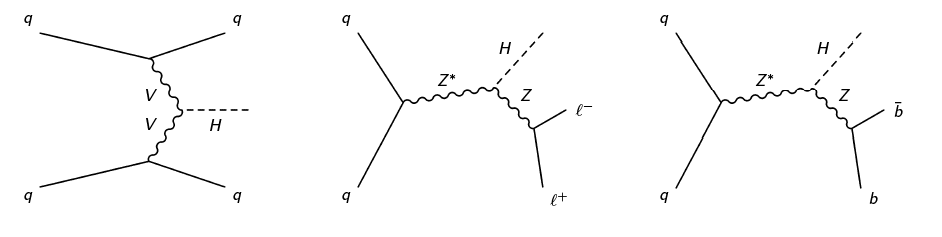
\includegraphics[width=\textwidth]{TalkPics/invcomb021213/feyndiags}
%% \begin{fmfgraph*}(100,70)
%%         \fmfleft{i1,i2}
%%         \fmfright{o1,o2,o3}
%%         \fmf{fermion}{i1,v1,o1}
%%         \fmf{fermion}{i2,v2,o3}
%%         \fmf{phantom,tension=4/5}{v1,v2}
%%         \fmffreeze
%%         \fmf{photon,label=$W,,Z$}{v1,v3}
%%         \fmf{photon,label=$W,,Z$}{v2,v3}
%%         \fmf{dashes}{v3,o2}
%%         \fmflabel{$q$}{i1}
%%         \fmflabel{$q$}{i2}
%%         \fmflabel{$q$}{o1}
%%         \fmflabel{$q$}{o3}
%%         \fmflabel{$H$}{o2}
%%       \end{fmfgraph*}
}
\date{}
\begin{document}
\begin{fmffile}{hexotrig261015feyndiags}

%TITLE PAGE
\section{Title}
\begin{frame}
  \titlepage
  
\end{frame}

%!!CLOSURE TEST STATEMENT PU jet ID
%OUTLINE
\begin{frame}
  \frametitle{Reminder}
  \scriptsize
  \begin{block}{}
    \begin{itemize}
      \item Presented trigger efficiency measurements using 1.28 fb$^{-1}$ to H-Exo last week
      \item Suggested to look at jet turn on in jet only trigger
      \item[-] Added pass/fail information for HLT\_DiPFJetAve40 and HLT\_PFHT750\_4JetPt50
      \item Also wanted to look at offline vs online jet $p_{T}$
      \item[-] Addedd HLT pf jets matched to offline leading jets
      \item[-] Added calo jets matched to offline leading jets
      \item[-] Trigger objects only present when event passes trigger
    \end{itemize}
  \end{block}
\end{frame}

\begin{frame}
  \frametitle{Offline to online resolution: PF}
  \begin{block}{}
    \scriptsize
    \begin{itemize}      
    \item Compare offline and online jet $p_{T}$
    \item Trigger cut is at 40 GeV
    \end{itemize}
  \end{block}
  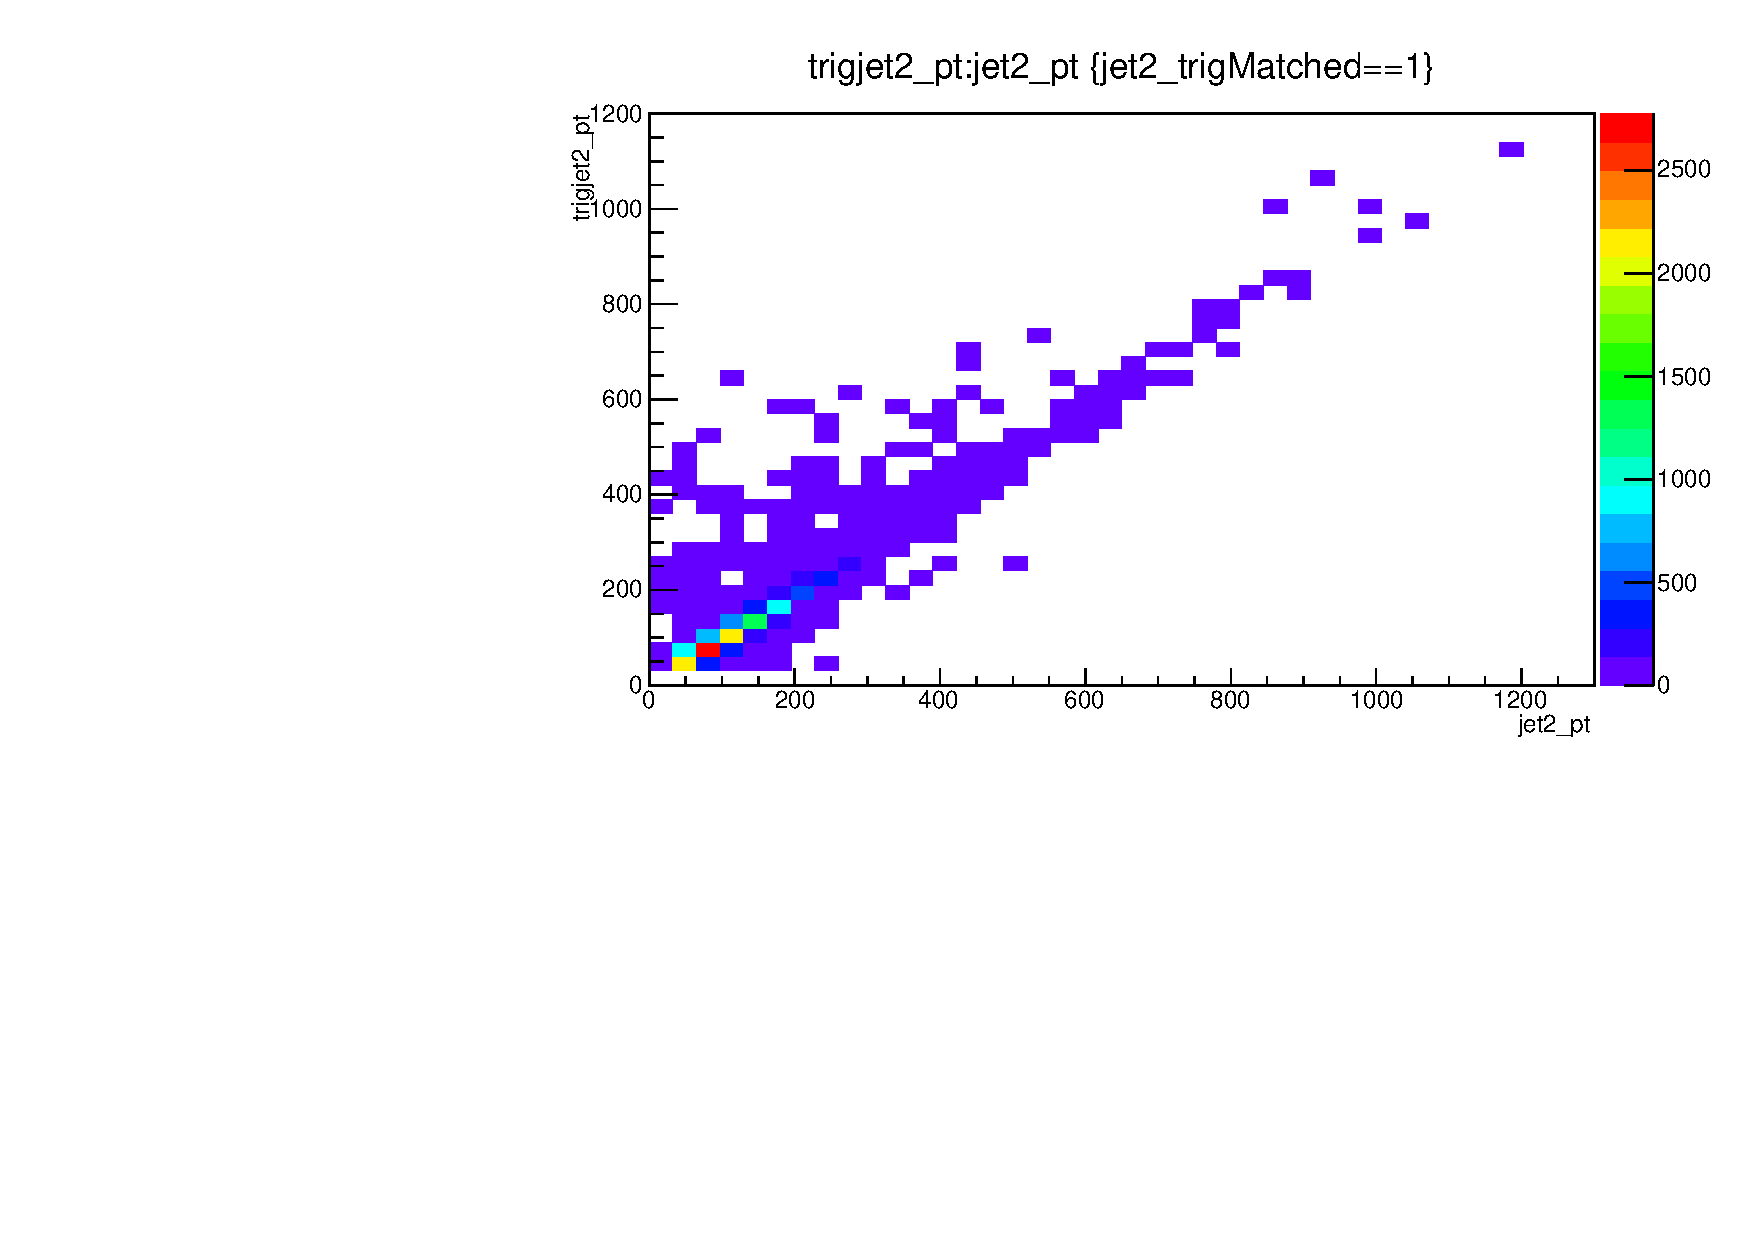
\includegraphics[width=.5\textwidth]{TalkPics/trigeff021115/trigeffstudies/jet2trigresponse.pdf}
  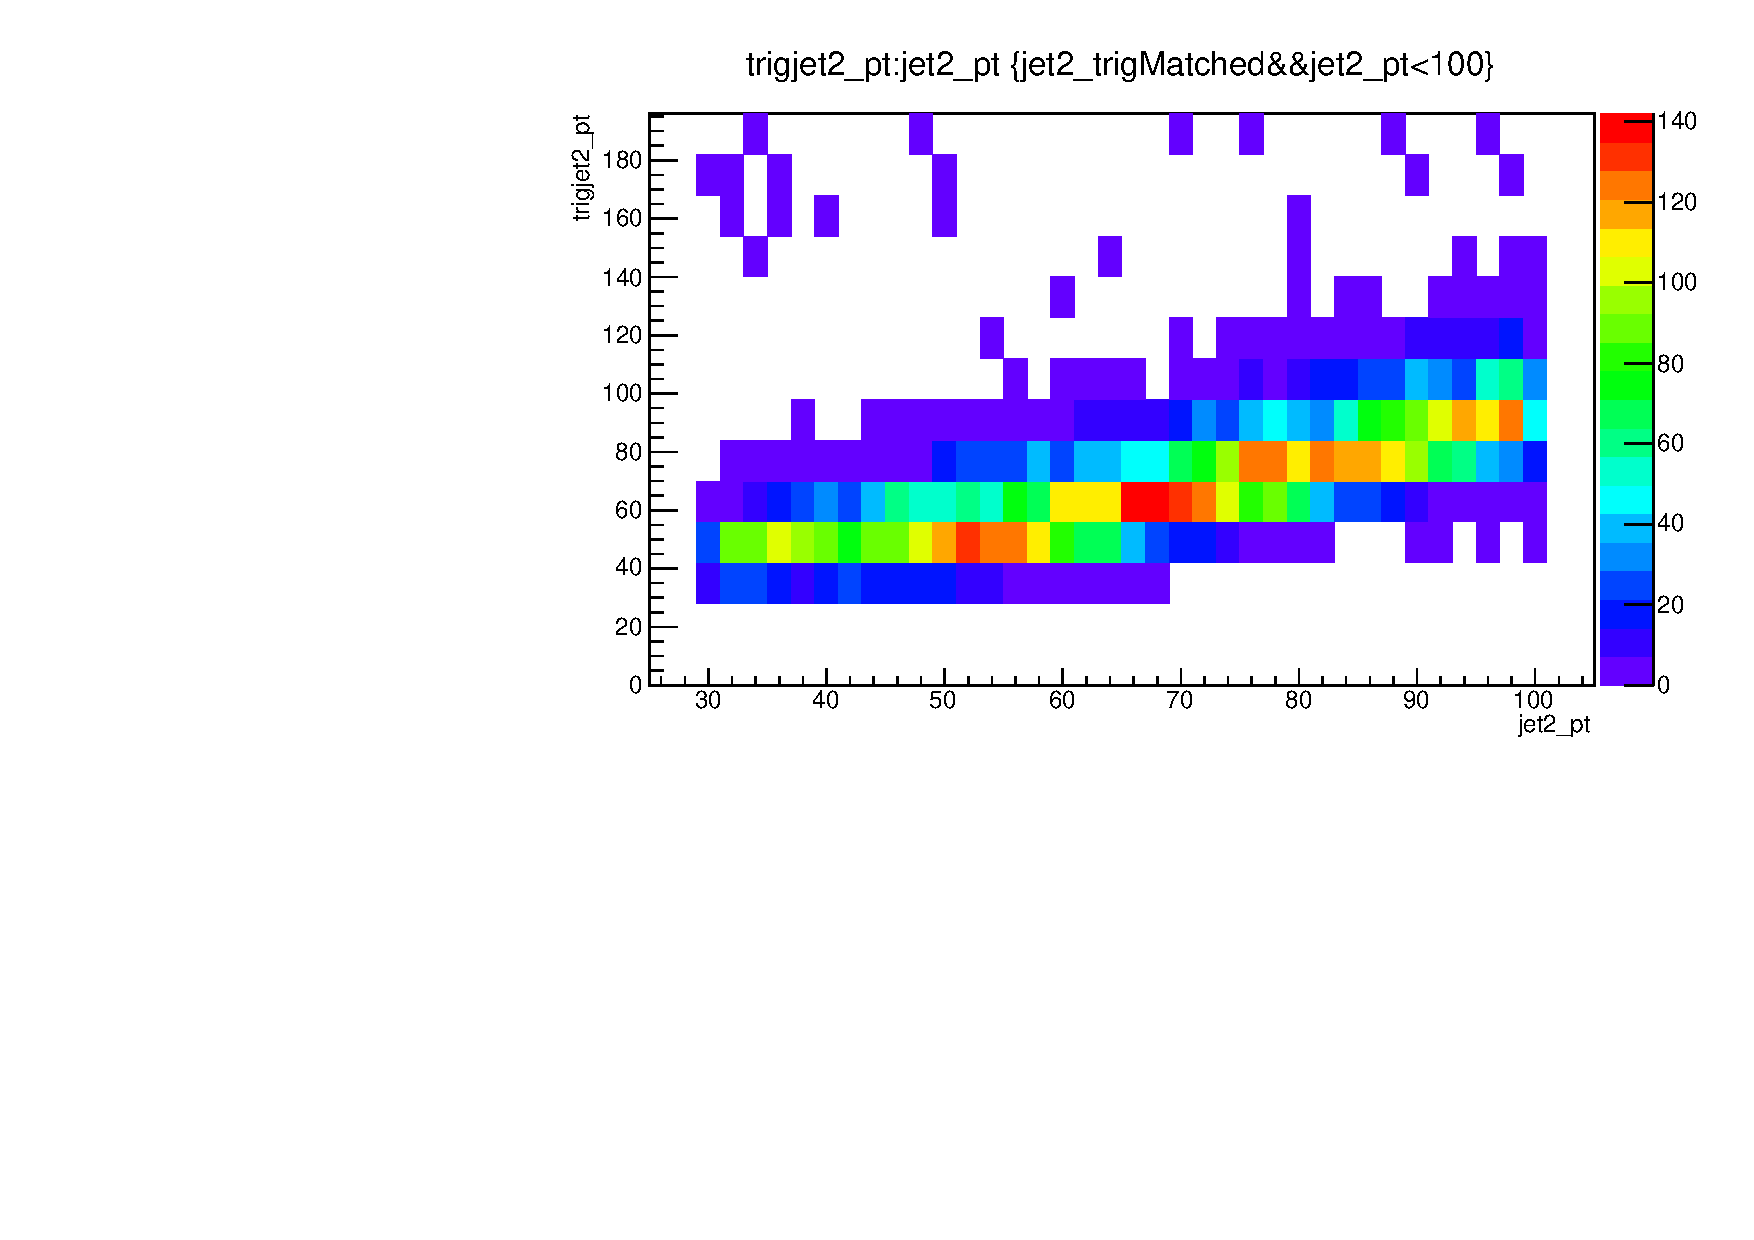
\includegraphics[width=.5\textwidth]{TalkPics/trigeff021115/trigeffstudies/jet2trigresponsept<100.pdf}
\end{frame}

\begin{frame}
  \frametitle{Offline to online resolution: PF}
  \begin{block}{}
    \scriptsize
    \begin{itemize}      
    \item Compare offline and online jet $p_{T}$
    \item[-] Left plot is for all jets right is for $p_{T}<50$ GeV
    \item Trigger cut is at 40 GeV
    \end{itemize}
  \end{block}
  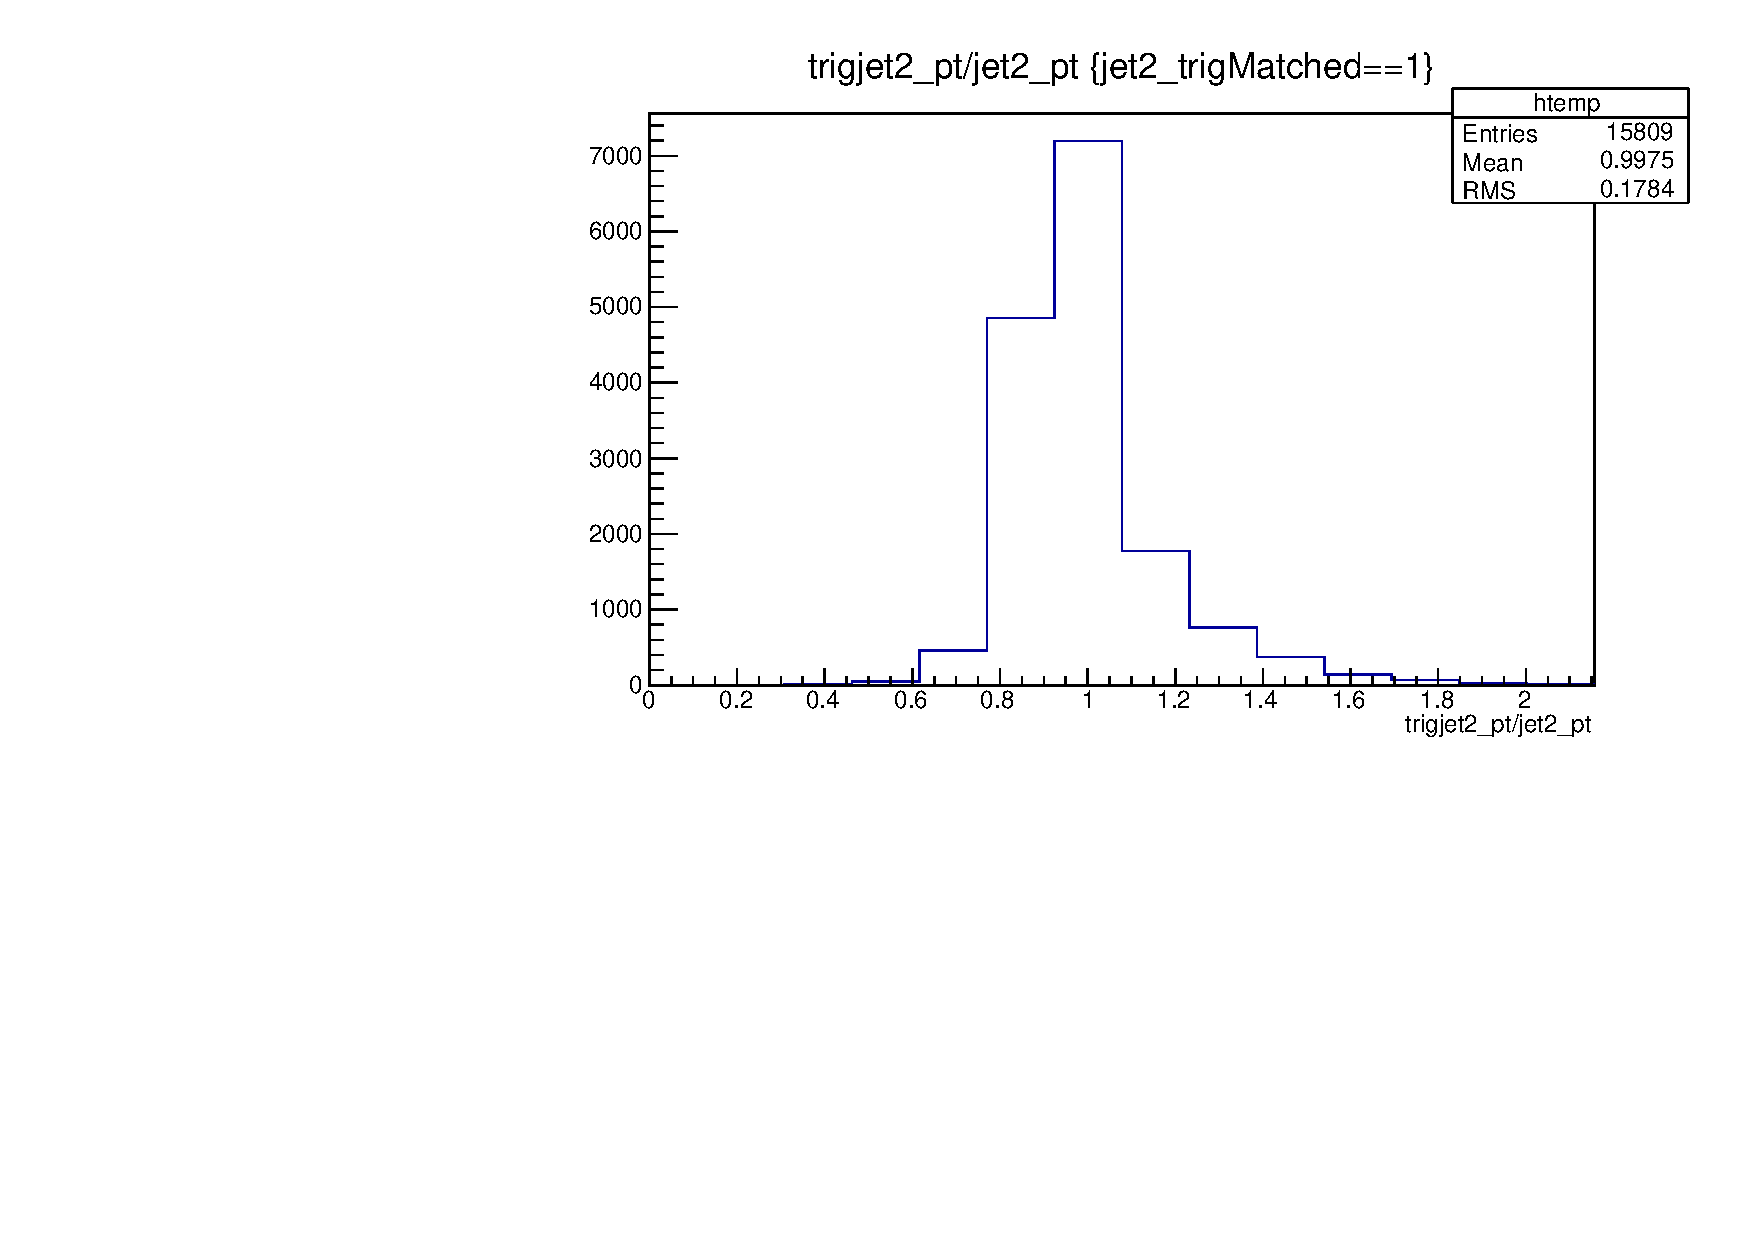
\includegraphics[width=.5\textwidth]{TalkPics/trigeff021115/trigeffstudies/jet2resolution.pdf}
  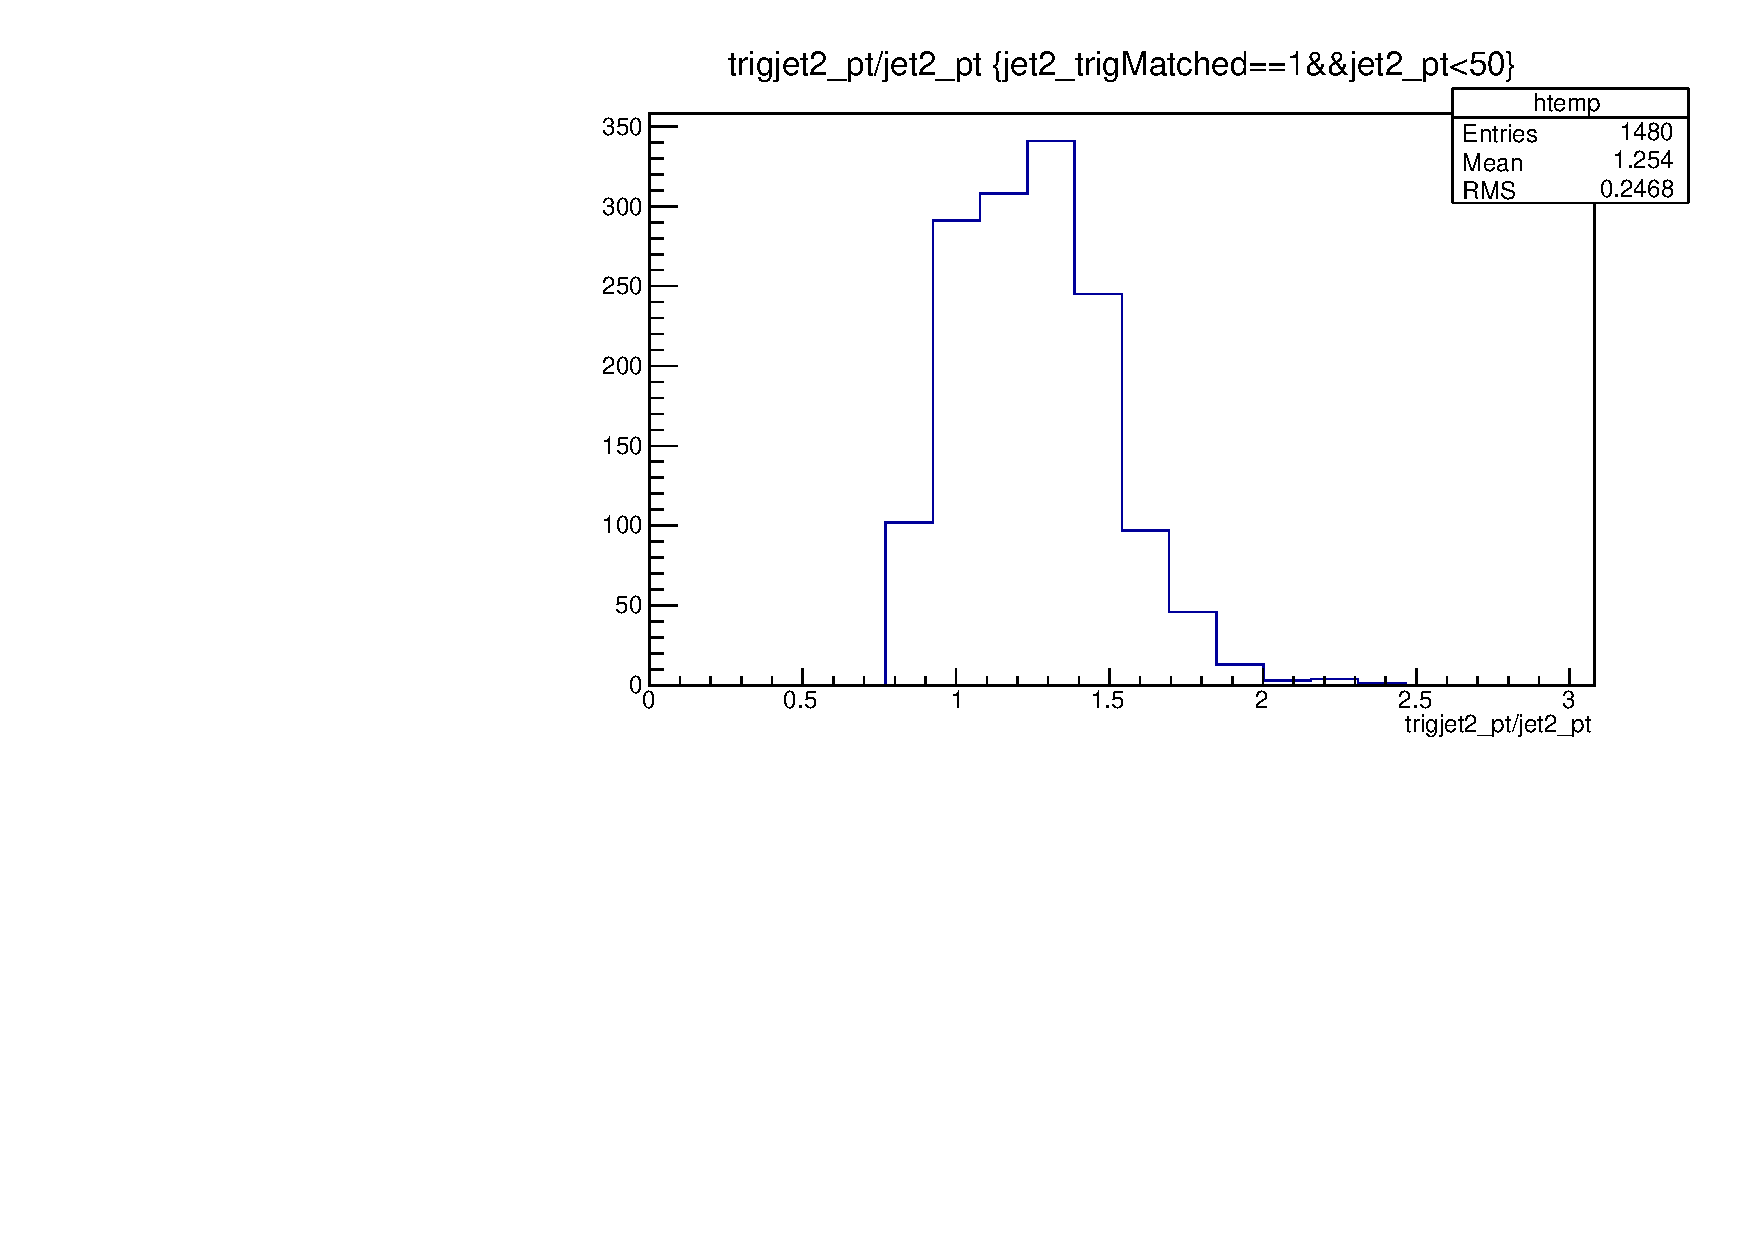
\includegraphics[width=.5\textwidth]{TalkPics/trigeff021115/trigeffstudies/jet2resolutionptbelow50.pdf}
\end{frame}



\begin{frame}
  \frametitle{Offline to online resolution: Calo}
  \begin{block}{}
    \scriptsize
    \begin{itemize}      
    \item We have a calo jet prefilter at 30 GeV
    \item It has been found that the wrong JEC was used at HLT in Run2015
    \item[-] \href{https://indico.cern.ch/event/456813/contribution/0/attachments/1178012/1704076/15-10-28_News_PPD.pdf}{Slides here}
    \item[-] this would have a larger effect on calo as the corrections are larger
    \end{itemize}
  \end{block}
  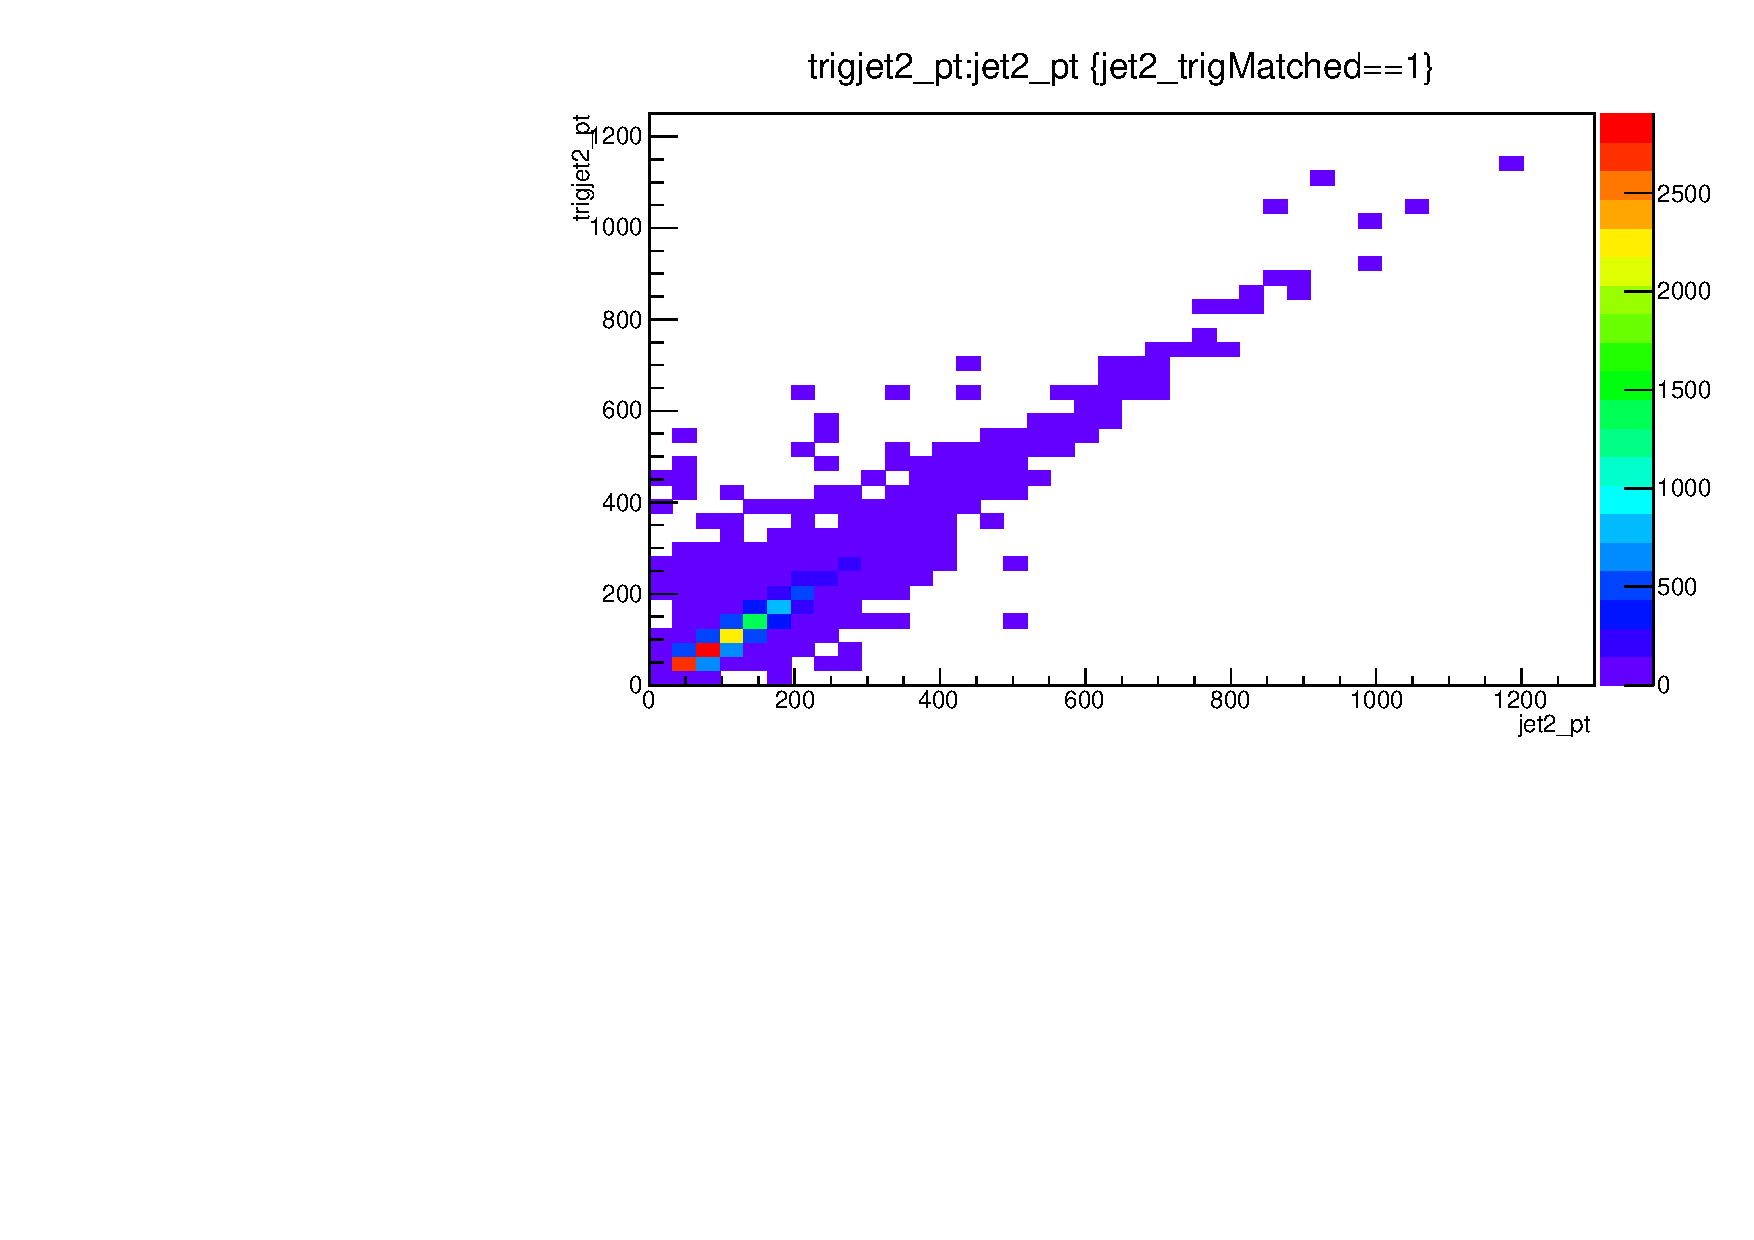
\includegraphics[width=.5\textwidth]{TalkPics/trigeff021115/trigeffstudies/jet2calotrigresponse.pdf}
  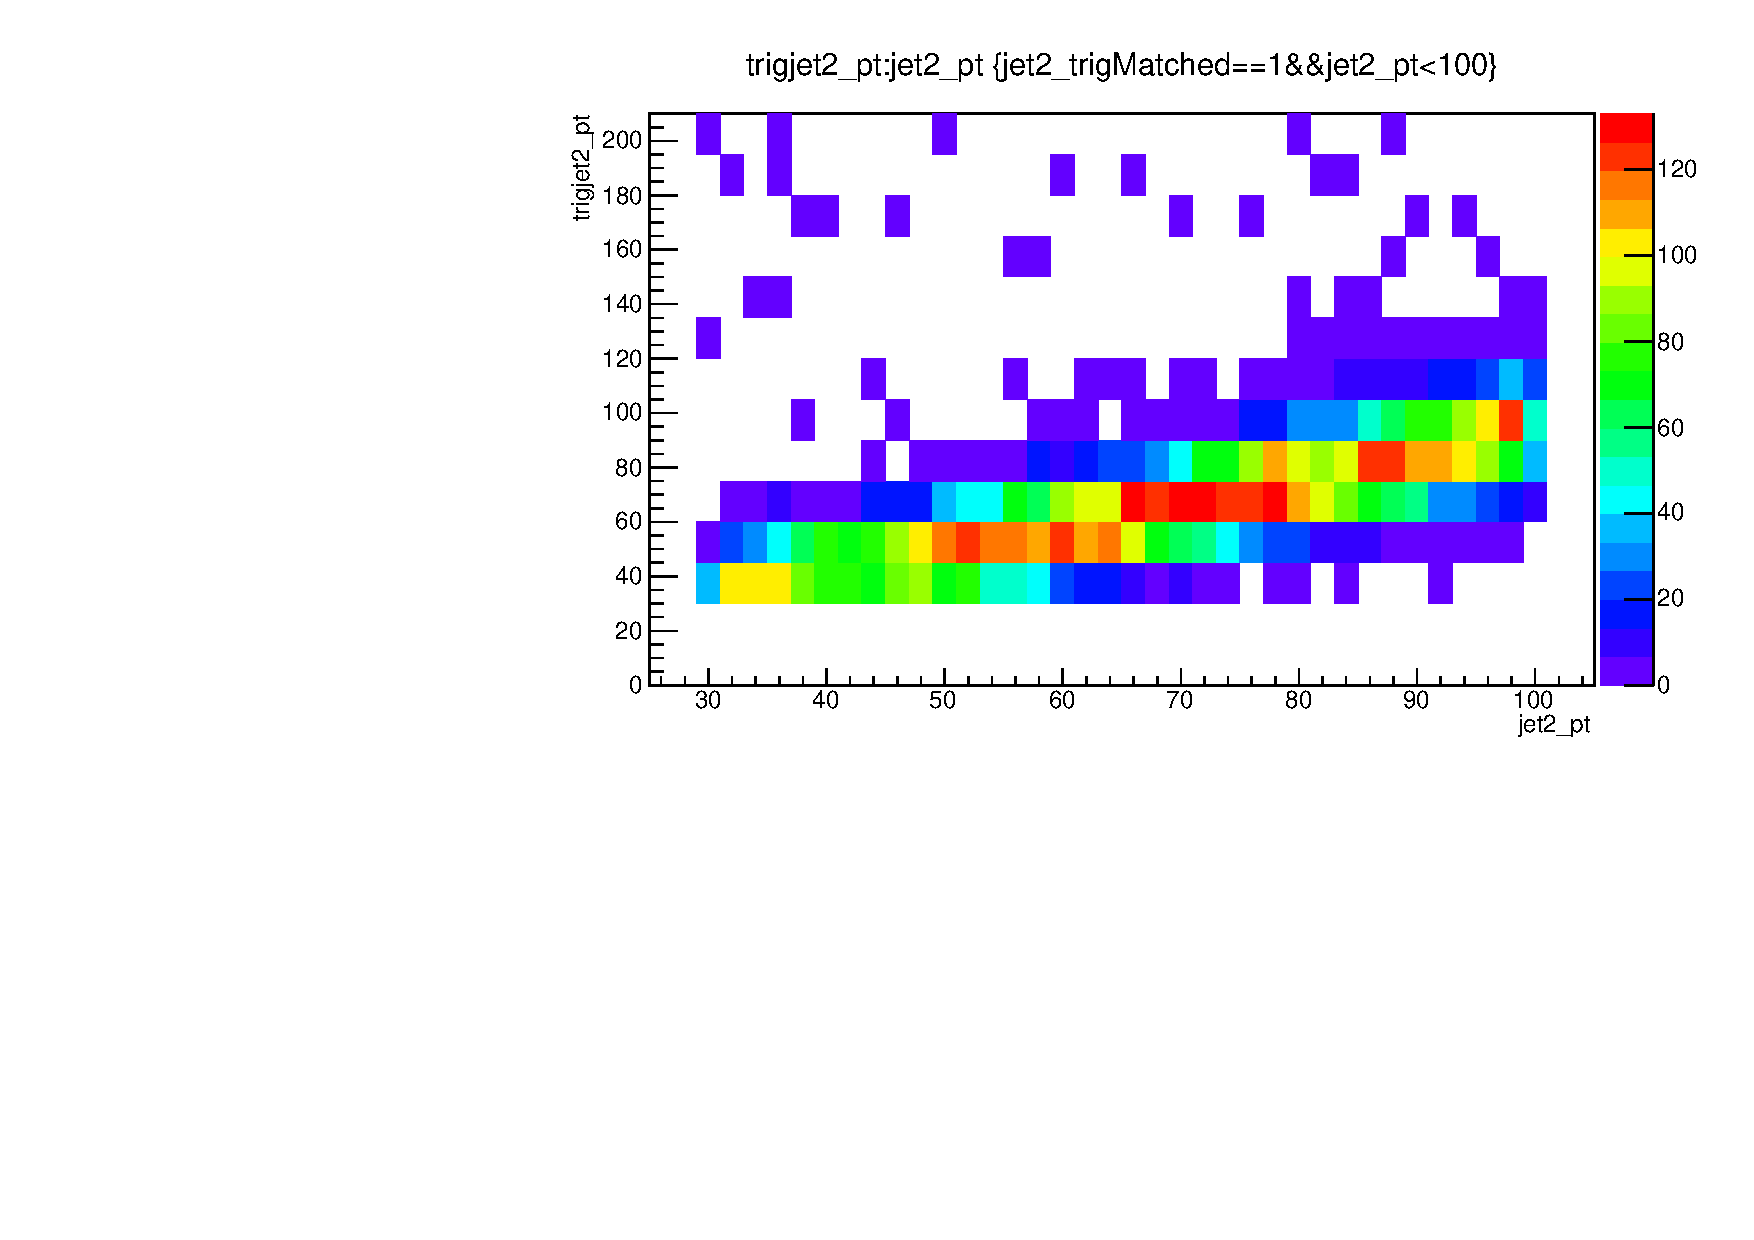
\includegraphics[width=.5\textwidth]{TalkPics/trigeff021115/trigeffstudies/jet2calotrigresponsept<100.pdf}
\end{frame}

\begin{frame}
  \frametitle{Offline to online resolution: PF}
  \begin{block}{}
    \scriptsize
    \begin{itemize}      
    \item We have a calo jet prefilter at 30 GeV
    \item It has been found that the wrong JEC was used at HLT in Run2015
    \item[-] \href{https://indico.cern.ch/event/456813/contribution/0/attachments/1178012/1704076/15-10-28_News_PPD.pdf}{Slides here}
    \item[-] this would have a larger effect on calo as the corrections are larger
    \item Left plot is for all jets right is for $p_{T}<50$ GeV
    \end{itemize}
  \end{block}
  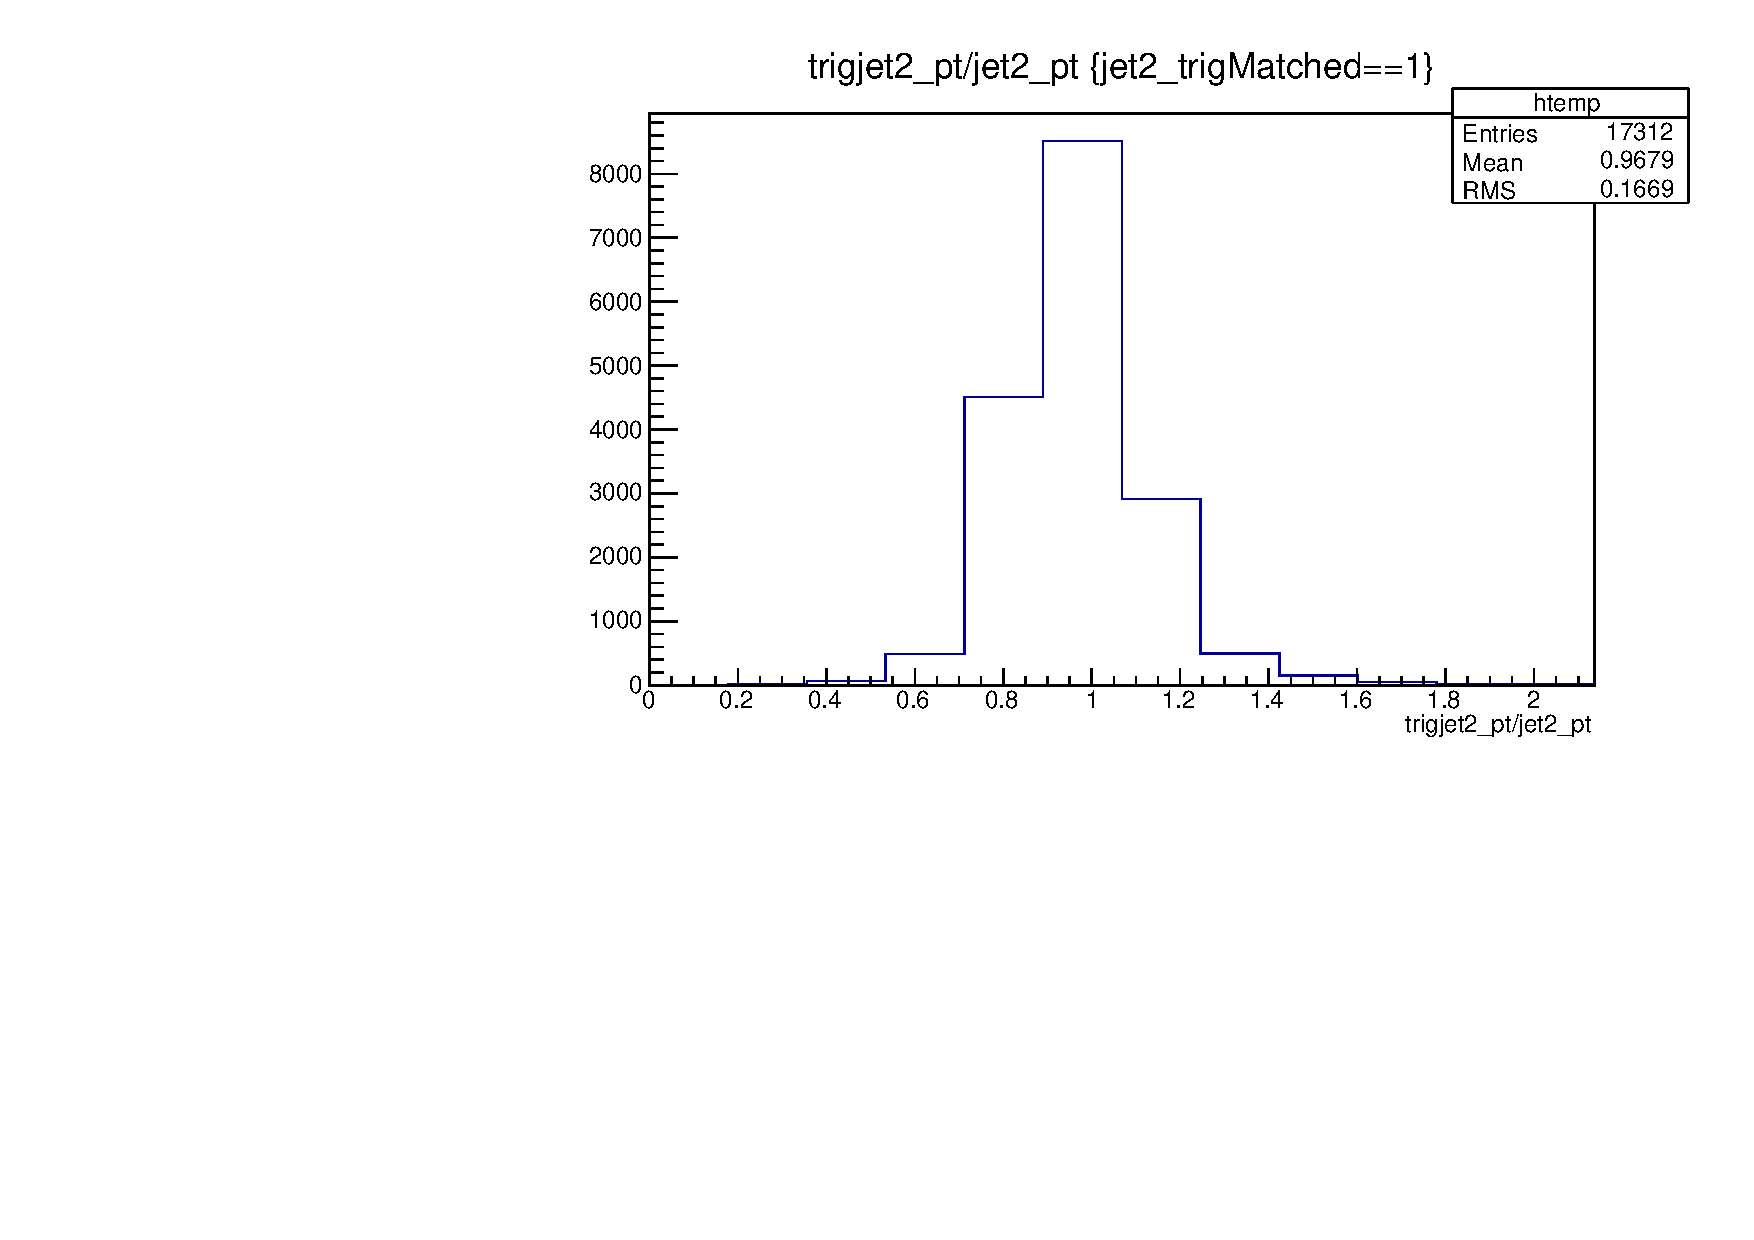
\includegraphics[width=.5\textwidth]{TalkPics/trigeff021115/trigeffstudies/jet2caloresolution.pdf}
  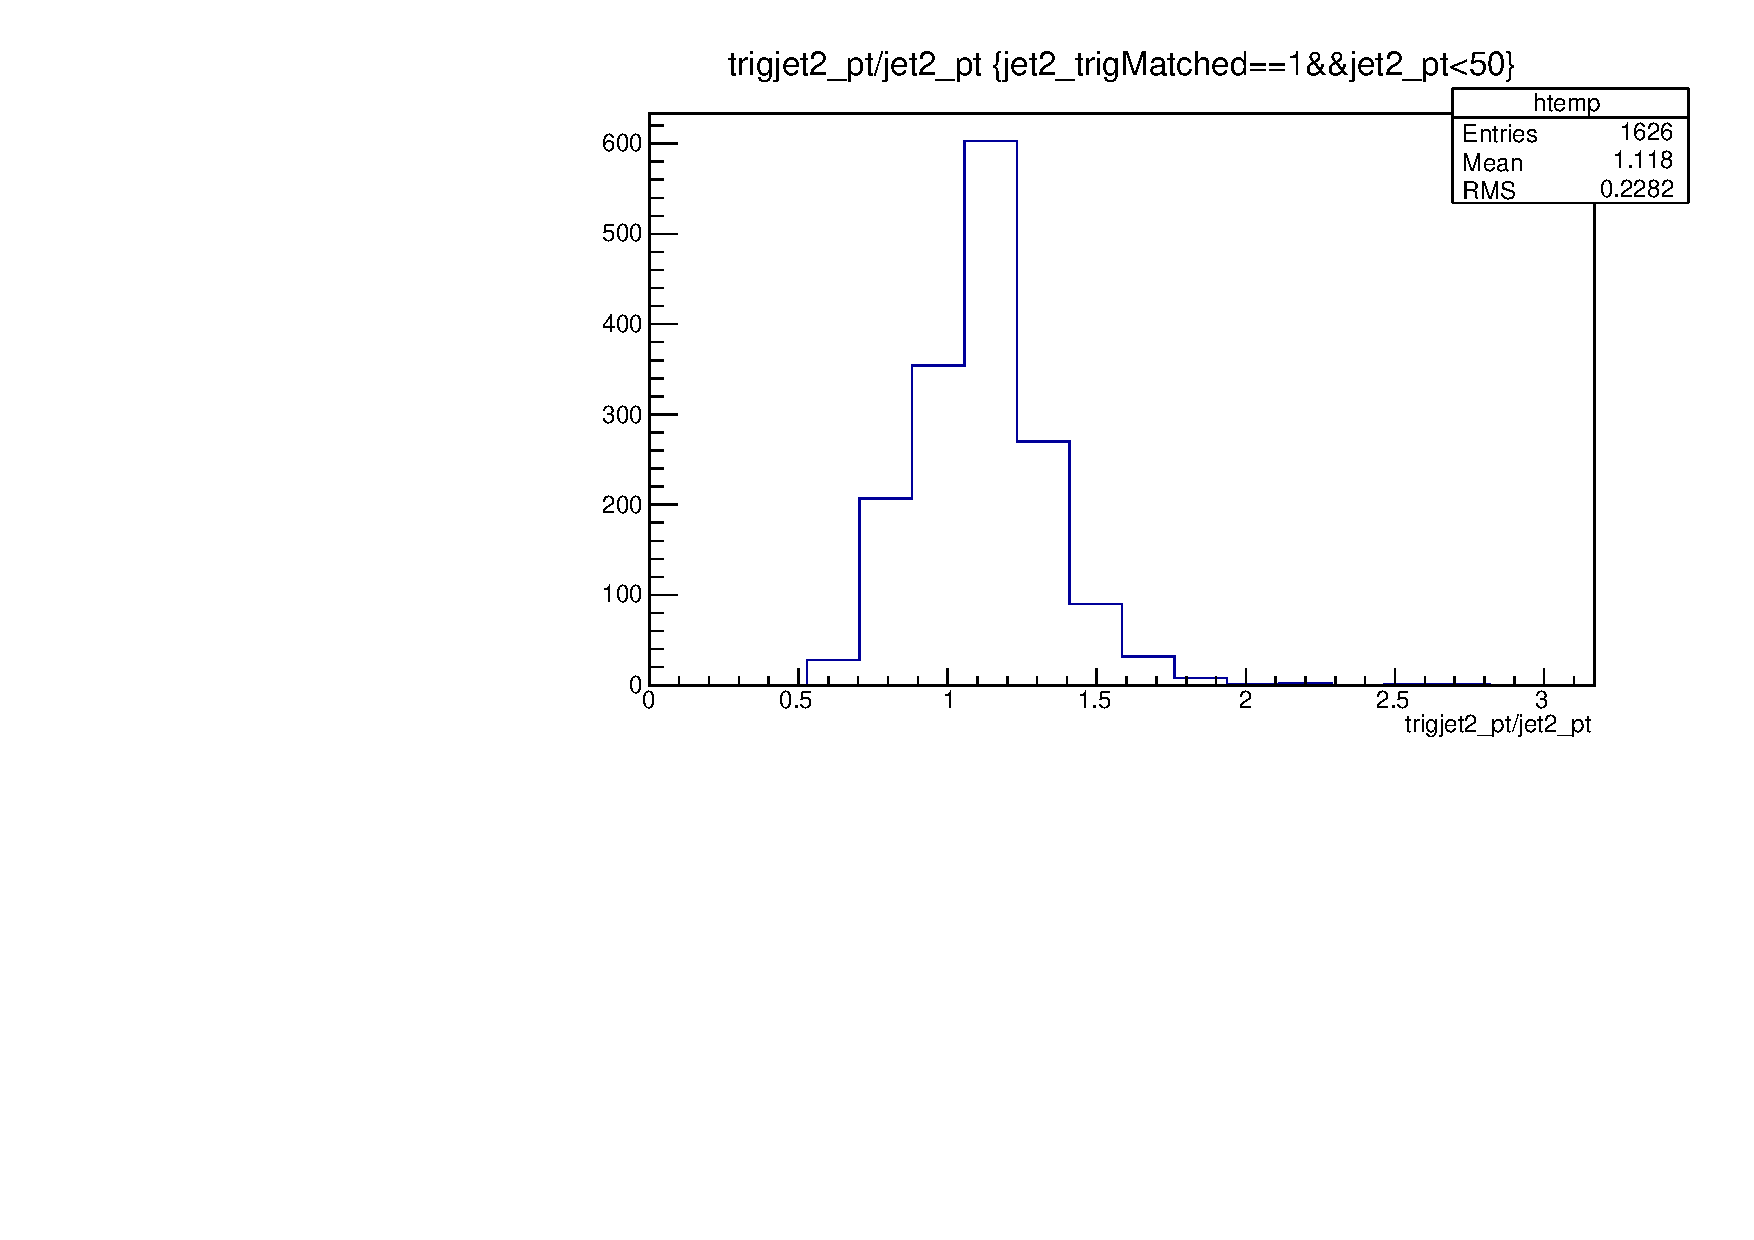
\includegraphics[width=.5\textwidth]{TalkPics/trigeff021115/trigeffstudies/jet2caloresolutionptbelow50.pdf}
\end{frame}


\begin{frame}
  \frametitle{Turn on in jet only trigger}
  \scriptsize
  \vspace{-.2cm}
  \begin{block}{}
    \begin{itemize}
    \item Have pass/fail information for HLT\_DiPFJetAve40 and HLT\_PFHT750\_4JetPt50
    \item[-] HLT\_DiPFJetAve40 is so prescaled no events pass in singlemuon sample
    \item Study turn on in HLT\_PFHT750\_4JetPt50
    \item[-] HT turn on is 90\% efficient at 1200 so cut there
    \item Over 90\% efficient by 60 GeV
    \item No calo jet pt prefilter
    \end{itemize}
  \end{block}
  \centering
  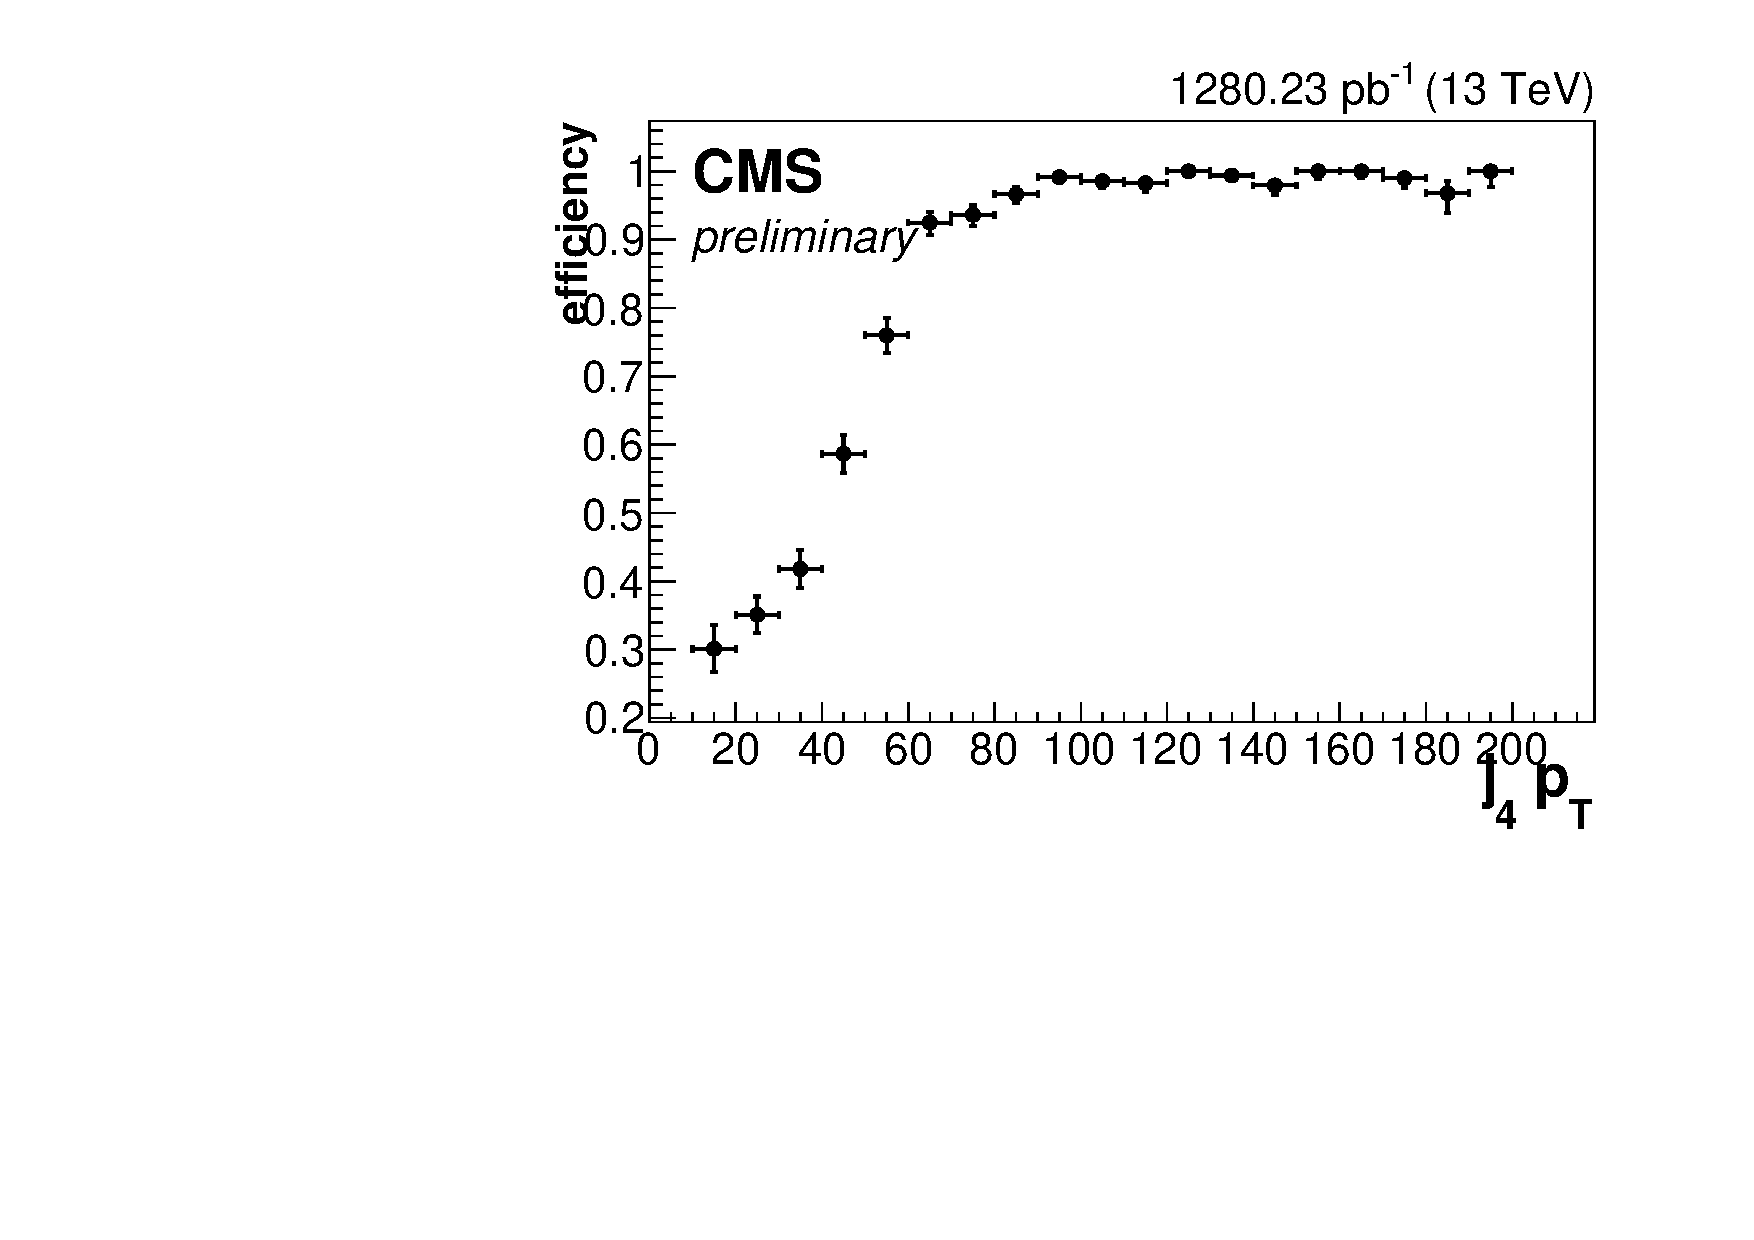
\includegraphics[width=.5\textwidth]{TalkPics/trigeffandpheno041115/nunu_jet4_pt.pdf}
\end{frame}

\begin{frame}
  \frametitle{Trigger efficiencies latest golden JSON}
  \scriptsize
  \begin{block}{}
    \begin{itemize}
    \item HLT\_DiPFJet40\_DEta3p5\_MJJ600\_PFMETNoMu140
    \item Use SingleMuon dataset
    \item METnoMu$>300$ GeV, DiPFJet$>80$ GeV, $\Delta\eta_{jj}>3.6$, $M_{jj}>$600
    \end{itemize}
  \end{block}
  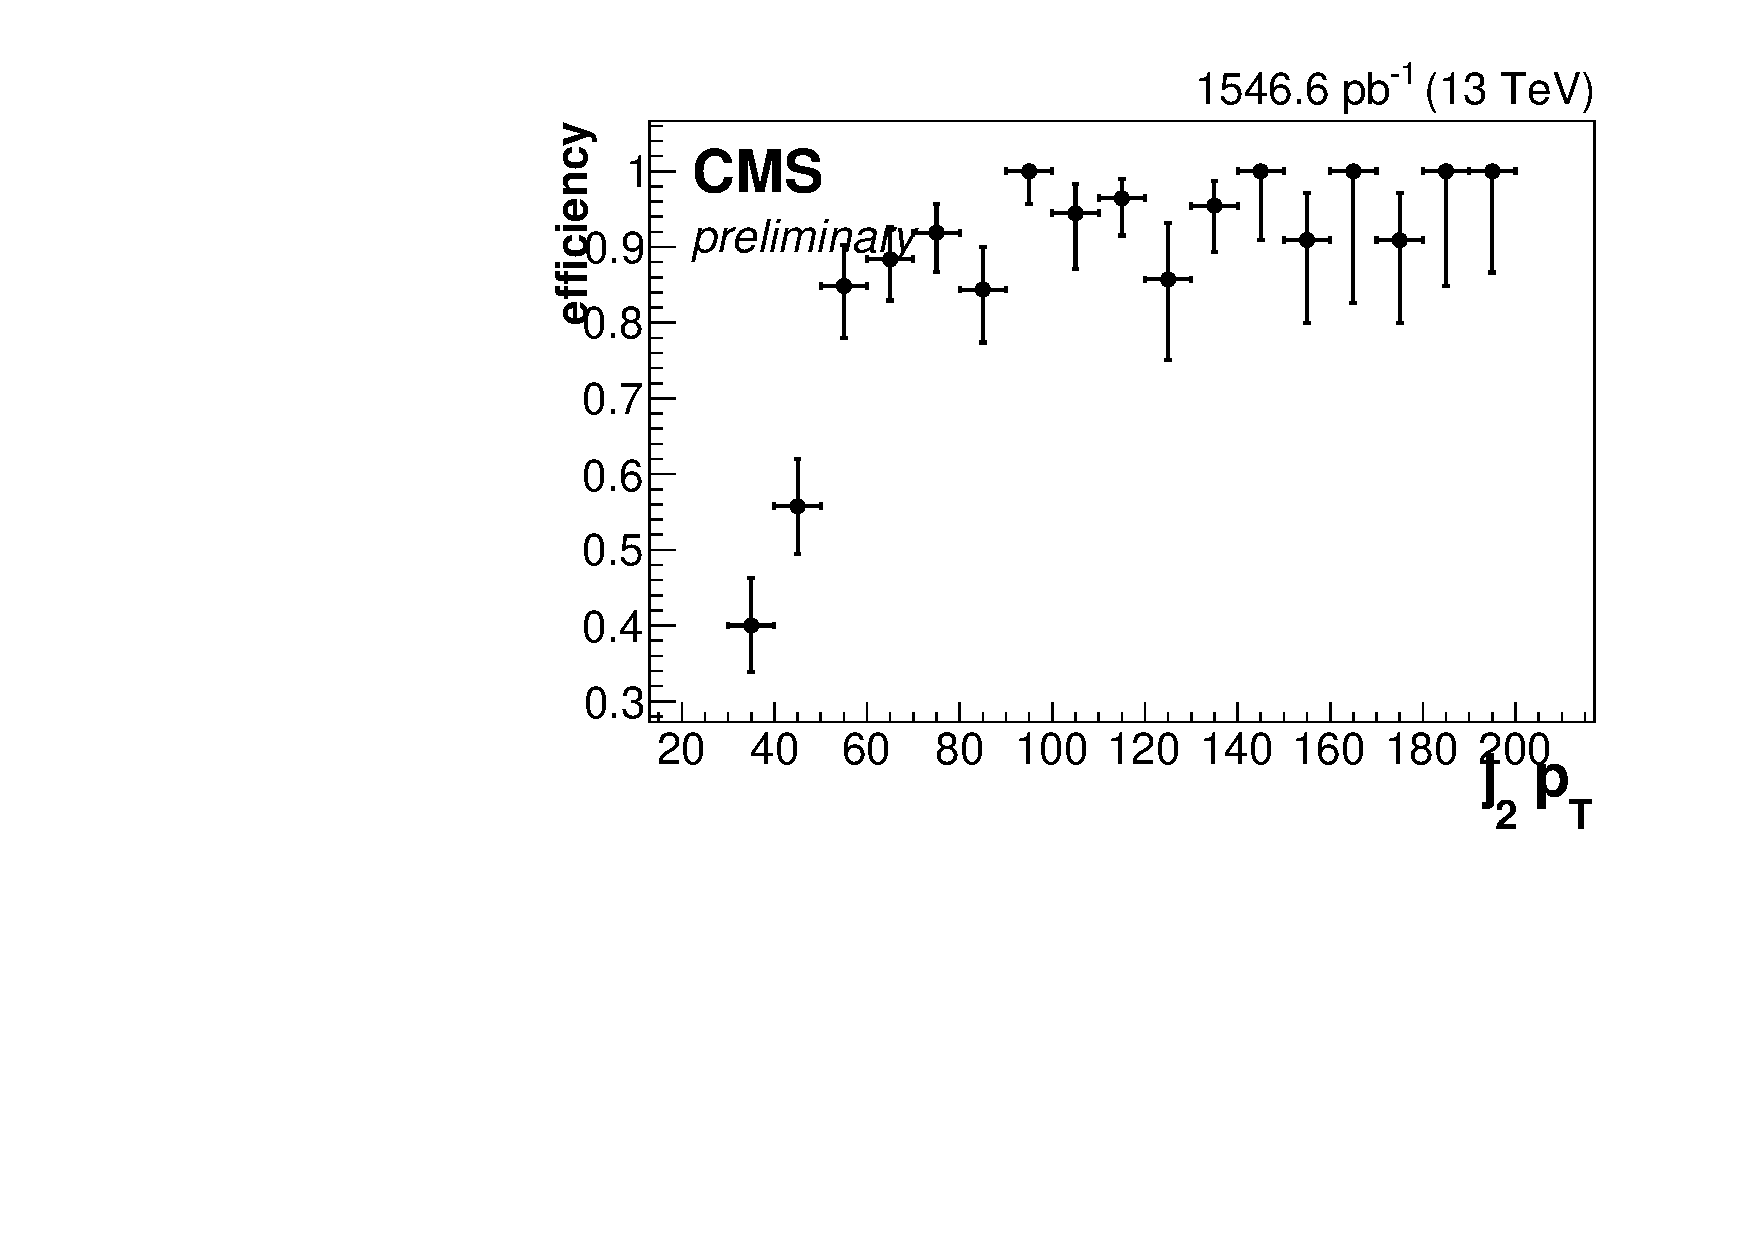
\includegraphics[width=.5\textwidth]{TalkPics/trigeffandpheno041115/nunu_jet2_pt.pdf}
  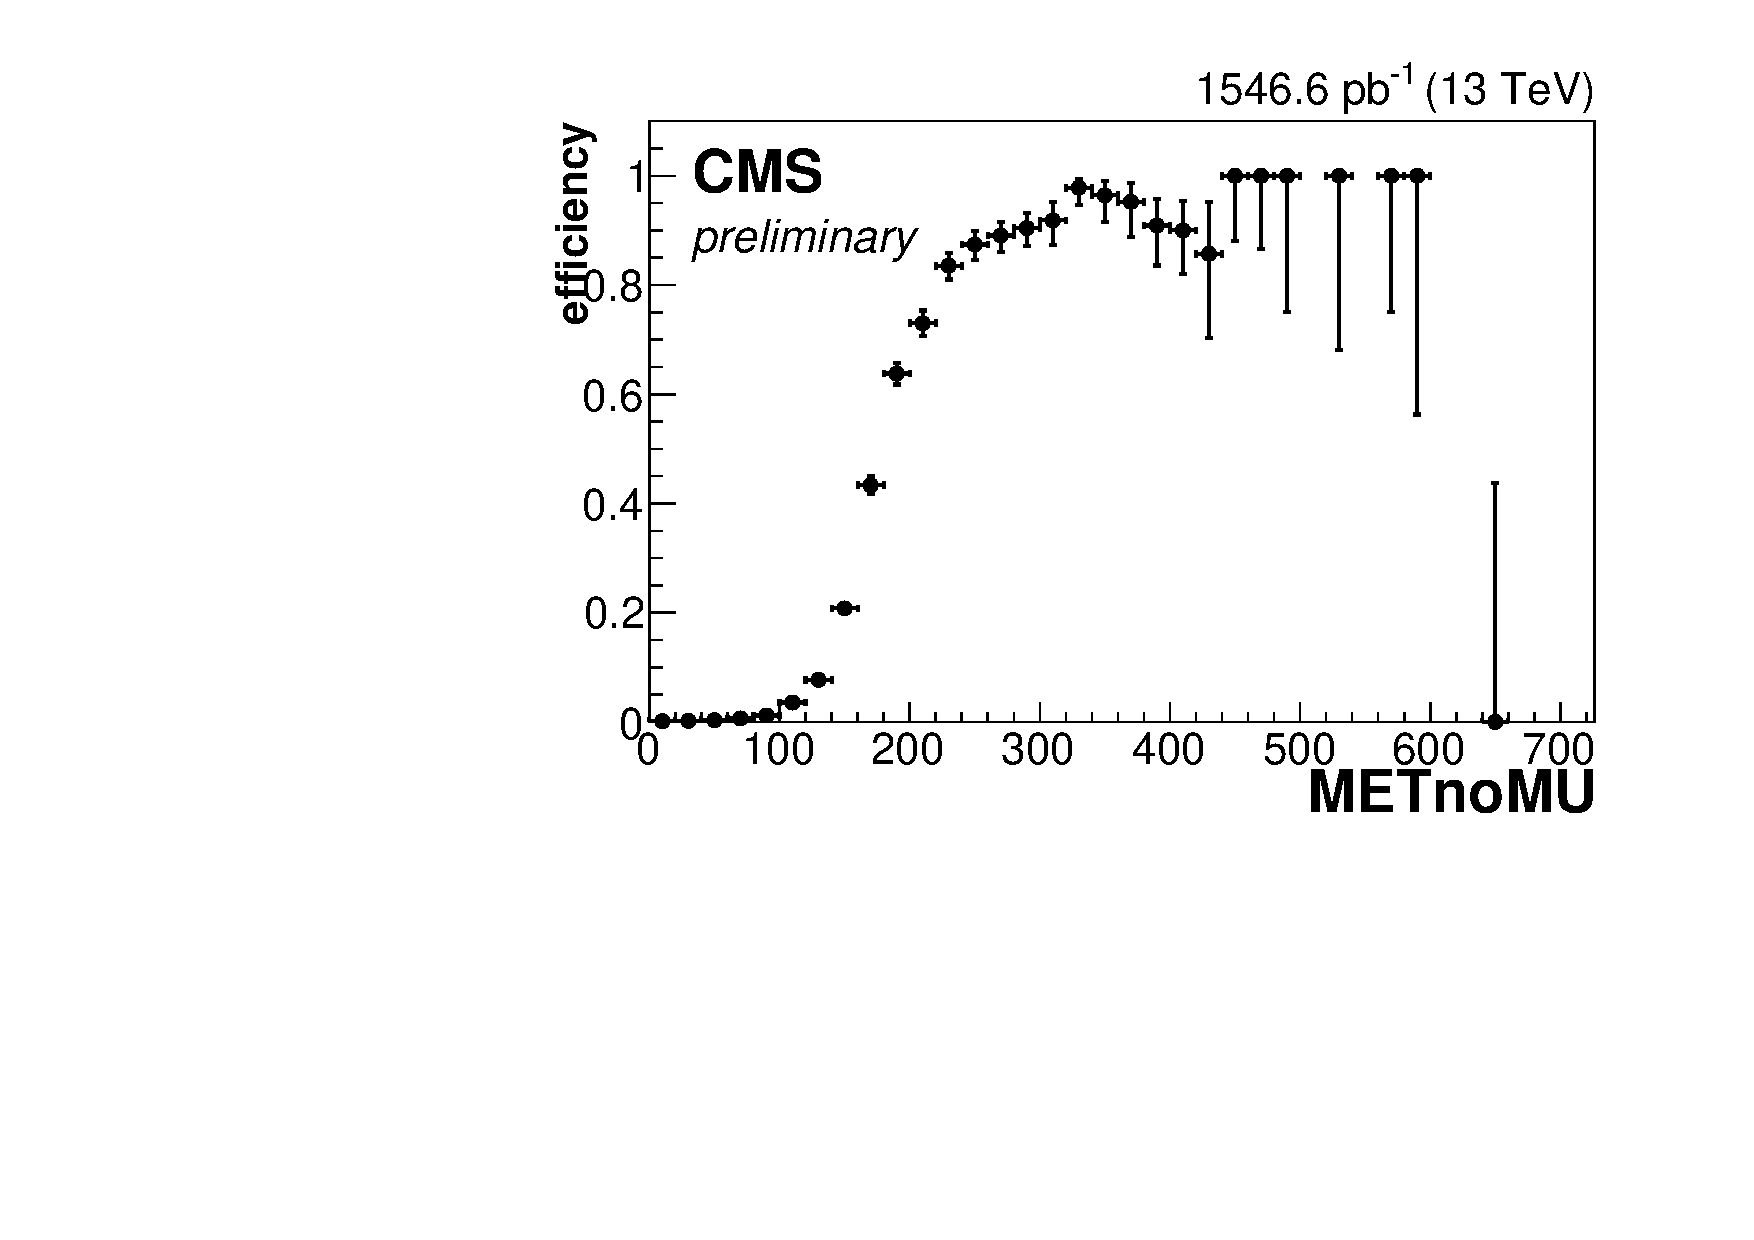
\includegraphics[width=.5\textwidth]{TalkPics/trigeffandpheno041115/nunu_metnomuons.pdf}
\end{frame}

\begin{frame}
  \frametitle{Trigger efficiencies latest golden JSON}
  \scriptsize
  \begin{block}{}
    \begin{itemize}
    \item HLT\_DiPFJet40\_DEta3p5\_MJJ600\_PFMETNoMu140
    \item Use SingleMuon dataset
    \item METnoMu$>300$ GeV, DiPFJet$>80$ GeV, $\Delta\eta_{jj}>3.6$, $M_{jj}>$600
    \end{itemize}
  \end{block}
  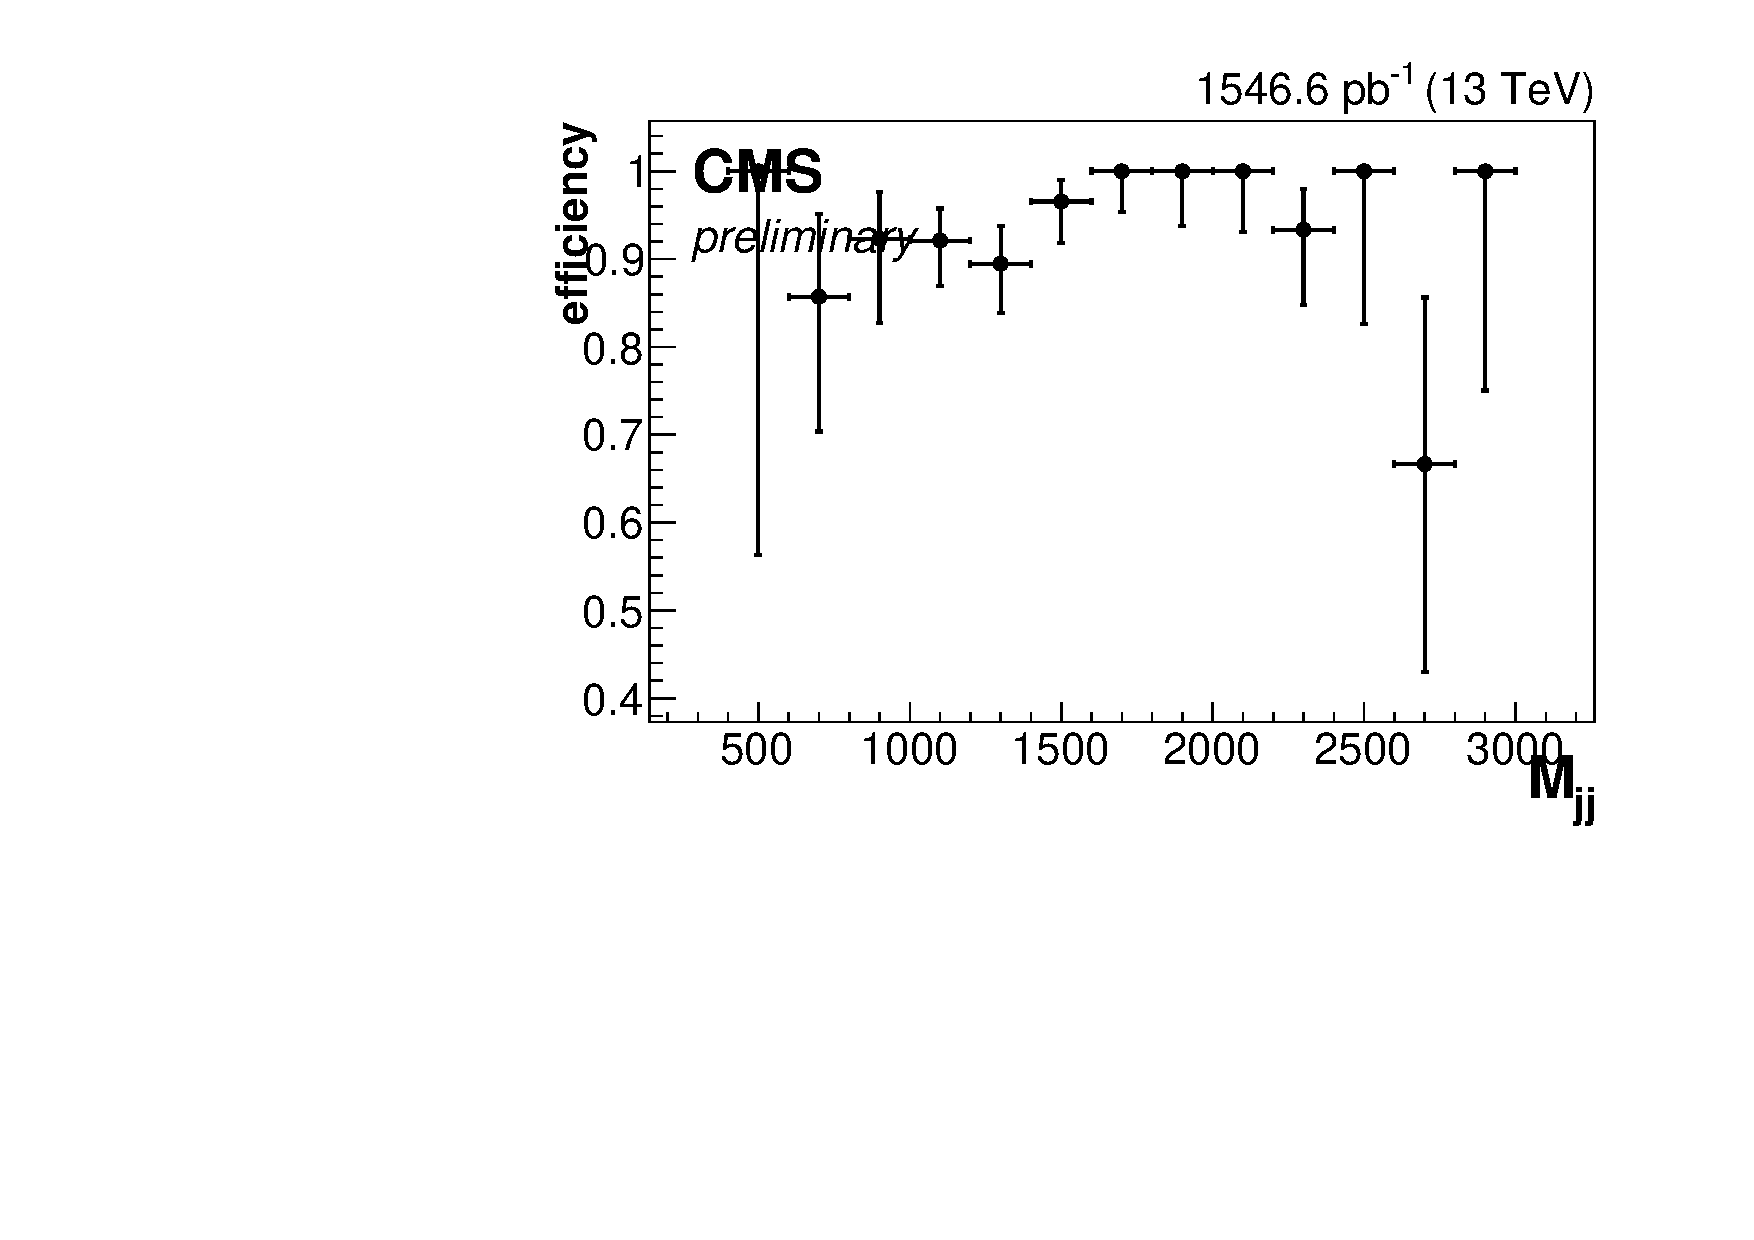
\includegraphics[width=.5\textwidth]{TalkPics/trigeffandpheno041115/nunu_dijet_M.pdf}
  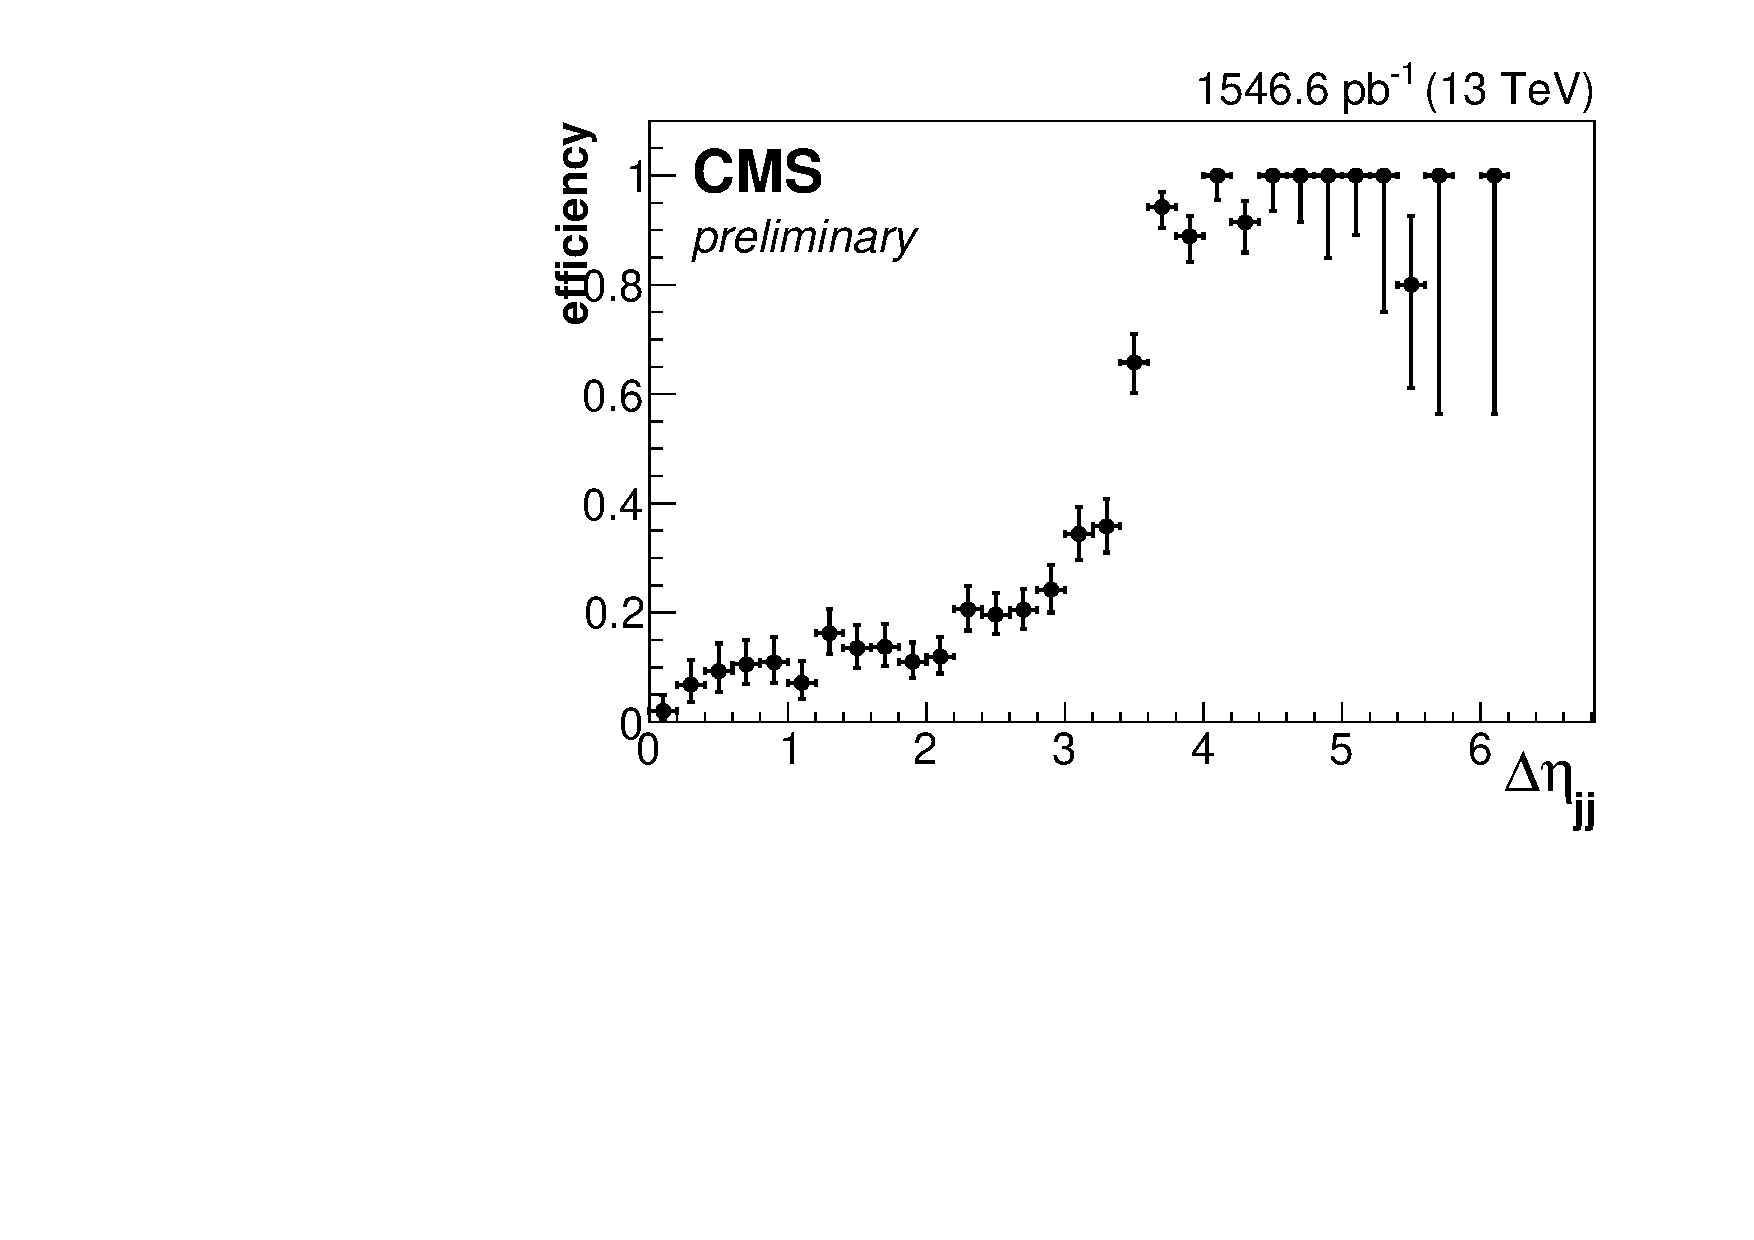
\includegraphics[width=.5\textwidth]{TalkPics/trigeffandpheno041115/nunu_dijet_deta.pdf}
\end{frame}

\begin{frame}
  \frametitle{13 TeV projections for pheno work}
  \scriptsize
  \begin{block}{}
    \begin{itemize}
    \item Scale all event yields by $\frac{\sigma_{13 TeV}}{\sigma_{8 TeV}}$
    \item[-] Cross-sections taken from public CMG tools repository
    \item Statistical errors scale with $\sqrt{yield}$
    \item Systematic errors constant
    \item[-] Will add scaling by $\sqrt{\mathcal{L}}$ in future
    \item Estimate 862 background events, 701 signal events
    \item Expected limit with 20 (2) fb$^{-1}$ \textcolor{red}{26 (51)\%}
    \end{itemize}
  \end{block}
\end{frame}

\begin{frame}
  \frametitle{Summary}
  \label{lastframe}
  \scriptsize
  \begin{block}{}
    \begin{itemize}
    \item Calo prefilter + wrong JEC possible candidate for slow trigger turn on but needs more investigation
    \item[-] Jim reemulating trigger on raw data so we can study events failing trigger
    \item CSC halo filter v1 list of veto events came out over the weekend
    \item[-] Need to switch to this but not expected to have a big effect
    \item We have a model of the analysis at 13 TeV which we can use for the phenomenology work
    \end{itemize}
  \end{block}
  \centering
\end{frame}

%UPDATED BACKUP
\begin{frame}
  \frametitle{Backup}
\end{frame}

\begin{frame}
\end{frame}

\end{fmffile}
\end{document}
